%%%
%
% $Autor: Wings $
% $Datum: 2021-05-14 $
% $Pfad: GitLab/MLEdgeComputer $
% $Dateiname: EthernetENC28J60.tex
% $Version: 4620 $
%
% !TeX spellcheck = de_DE/GB
% !TeX program = pdflatex
% !BIB program = biber/bibtex
% !TeX encoding = utf8
%
%%%






\chapter{Ethernetschnittstelle ENC28J60}

\begin{figure}
    \centering
    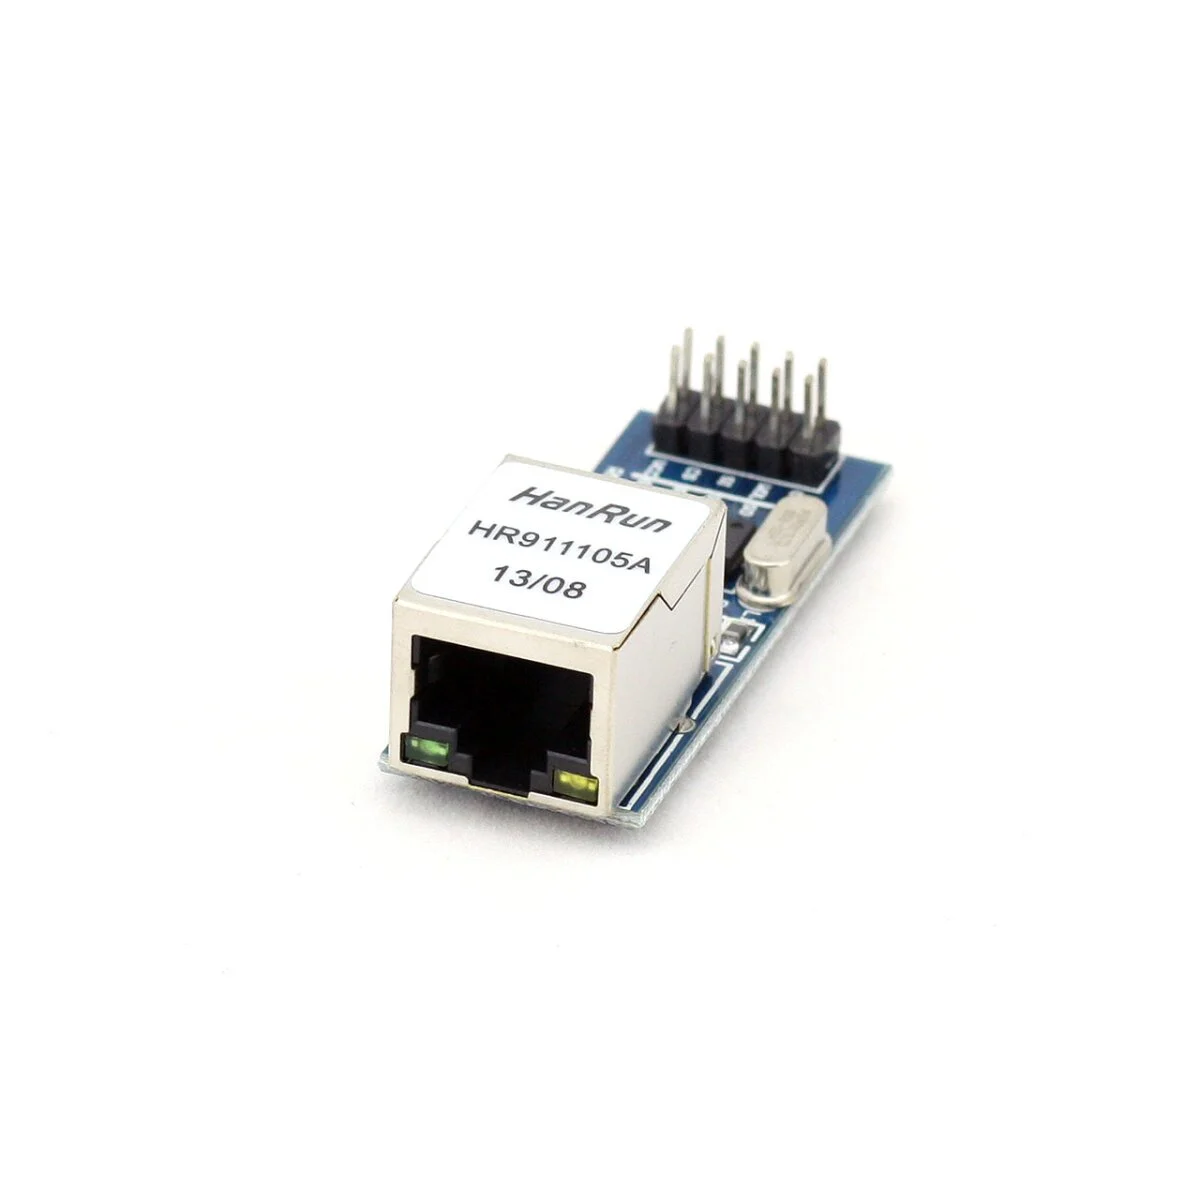
\includegraphics[width=7cm]{EthernetENC28J60/NetzwerkschnittstelleENC28J60}
    \caption{Netzwerkschnittstelle ENC28J60}
    \label{fig:NetzwerkschnittstelleENC28J60}
\end{figure}
Die ARD NET ENC28J60 Netzwerk- Schnittstelle \ref{fig:NetzwerkschnittstelleENC28J60} erweitert den Arduino über eine 10-Pin Buchsenleiste um eine Netzwerkschnittstelle für Ethernet- LAN. Dadurch wird es möglich einen Webserver aufzubauen oder Daten mit anderen Geräten auszutauschen. Das Modul kommuniziert mit dem Arduino über die SPI-Schnittstelle. In der SPI-Kommunikation werden Daten gleichzeitig übertragen und empfangen, wobei die synchronen Taktflanken das Timing für das Senden und Empfangen der Daten steuern. Aufgrund von Taktsignalen bis in den MHz Bereich, ist eine sehr hohe Rate der Datenübertragung möglich.  Damit die Schnittstelle benutzt werden kann, wird ein Arduino, wie der 33 BLE Sense, benötigt. Außerdem bedarf es Steckbrücken und ein Netzwerkkabel zum Router oder Switch. Über Stiftkontakte wird die Verbindung zum Arduino hergestellt. Diese Kontakte dienen zum einem dem Datenaustausch über die SPI-Schnittstelle, sowie der Spannungsversorgung und dem Massenanschluss. Damit das Modul betrieben werden kann, muss zusätzlich eine zugehörige “ENC28J60”- Bibliothek in Arduino IDE heruntergeladen und installiert werden. Die Bibliothek beinhaltet zugehörigen Beispiel Code, der unter “Examples” hinzugefügt wird. Dort müssen dann lediglich die Anschlusspins angepasst werden. \cite{Conrad:2024} \cite{Dhaker:2021}

\section{Netzadapter}

\begin{figure}[H]
    \centering
    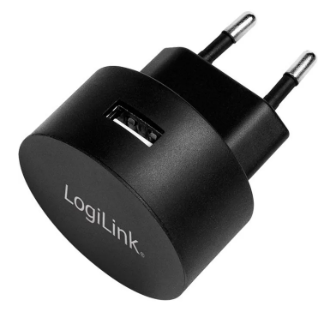
\includegraphics[width=7cm]{EthernetENC28J60/NetzadapterPA0217}
    \caption{Netzadapter PA0217}
    \label{fig:NetzadapterPA0217}
\end{figure}

Damit das automatisierte System mit Strom versorgt werden kann, benötigt es ein Netzadapter bzw. USB-Ladegerät. \ref{fig:NetzadapterPA0217} In diesem Fall handelt es sich um das “XTAR 5VWA USB-Ladegerät 5V 2,1A”. Die 5V im Titel beziehen sich auf den Output des Netzadapters. Dabei wird eine Stromstärke von 2100mA ausgegeben. Die Input-Spannung darf sich zwischen 100 V und 240 V Wechselstrom befinden. Bei dem Adapter handelt es sich um einen Eurostecker vom Typ C auf der einen Seite und einem weiblichen USB-Port vom Typ A auf der anderen Seite. Das Netzteil hat eine Tiefe von 80 mm, eine Höhe von 25 mm und eine Breite von 39 mm. \cite{LogiLink:2019}

\section{Test des  Ethernet-Shield ENC28J60} 

Der Code \FILE{LinkStatus.ino} \ref{Code:Python:File:LinkStatus}  überprüft die Verbindung zum ENC28J60 Ethernet Shield, welches per SPI Datenbus angeschlossen wird. Der Status wird jede Sekunde überprüft und über die serielle Schnittstelle ausgegeben. Der Sketch gibt $"$Unknown$"$ aus, wenn der Verbindungsstatus nicht bestimmt werden kann, $"$ON$"$ wenn das Kabel angeschlossen ist und $"$OFF$"$, wenn das Kabel nicht angeschlossen ist.

\begin{code}
    \lstinputlisting[language=c++]{../../Code/Arduino/EthernetENC28J60/LinkStatus.ino}
    \caption[Sketch \FILE{LinkStatus.ino}]{Der Sketch \FILE{LinkStatus.ino} in Arduino für das Microcontroller Board}
    \label{Code:Python:File:LinkStatus}   
\end{code}

\section{Test des Web Servers} 

Dieser Code \ref{Code:Python:File:TestENC} implementiert einen Webserver auf dem Arduino. Die Kommunikation zwischen Client und Server basiert auf dem HTTP-Protokoll. Er ermöglicht es dem Arduino Anfragen zu empfangen, zu verarbeiten und entsprechend zu antworten.
Zunächst wurde die Funktion durch Eingabe in der Adresszeile die LED anzusteuern hinzugefügt. Danach wurden Buttons auf der Website \ref{fig:GUI} per HTML Formular eingefügt. Nachdem dieser Schritt erfolgreich war, wurde der Code erweitert. Durch Betätigen der Schaltfläche $"$Bildschirmaufnahme$"$, soll der Void Capture aktiviert werden. Überprüft wurde dies zunächst durch das Aufleuchten der LED. Nachdem überprüft wurde, dass der Void Capture im Skript ausgeführt wird, sollte der Livestream erfolgen. Bevor die übertragenen Bytes ausgewertet wurden, trat das Problem auf, dass durch die große Datenmenge der Arbeitsspeicher im Arduino überlastet wurde. Im nächsten Schritt sollte dann die Datenübertragung als einzelne Bilder per Hexadezimal-String realisiert werden.

\begin{figure}
    \centering
    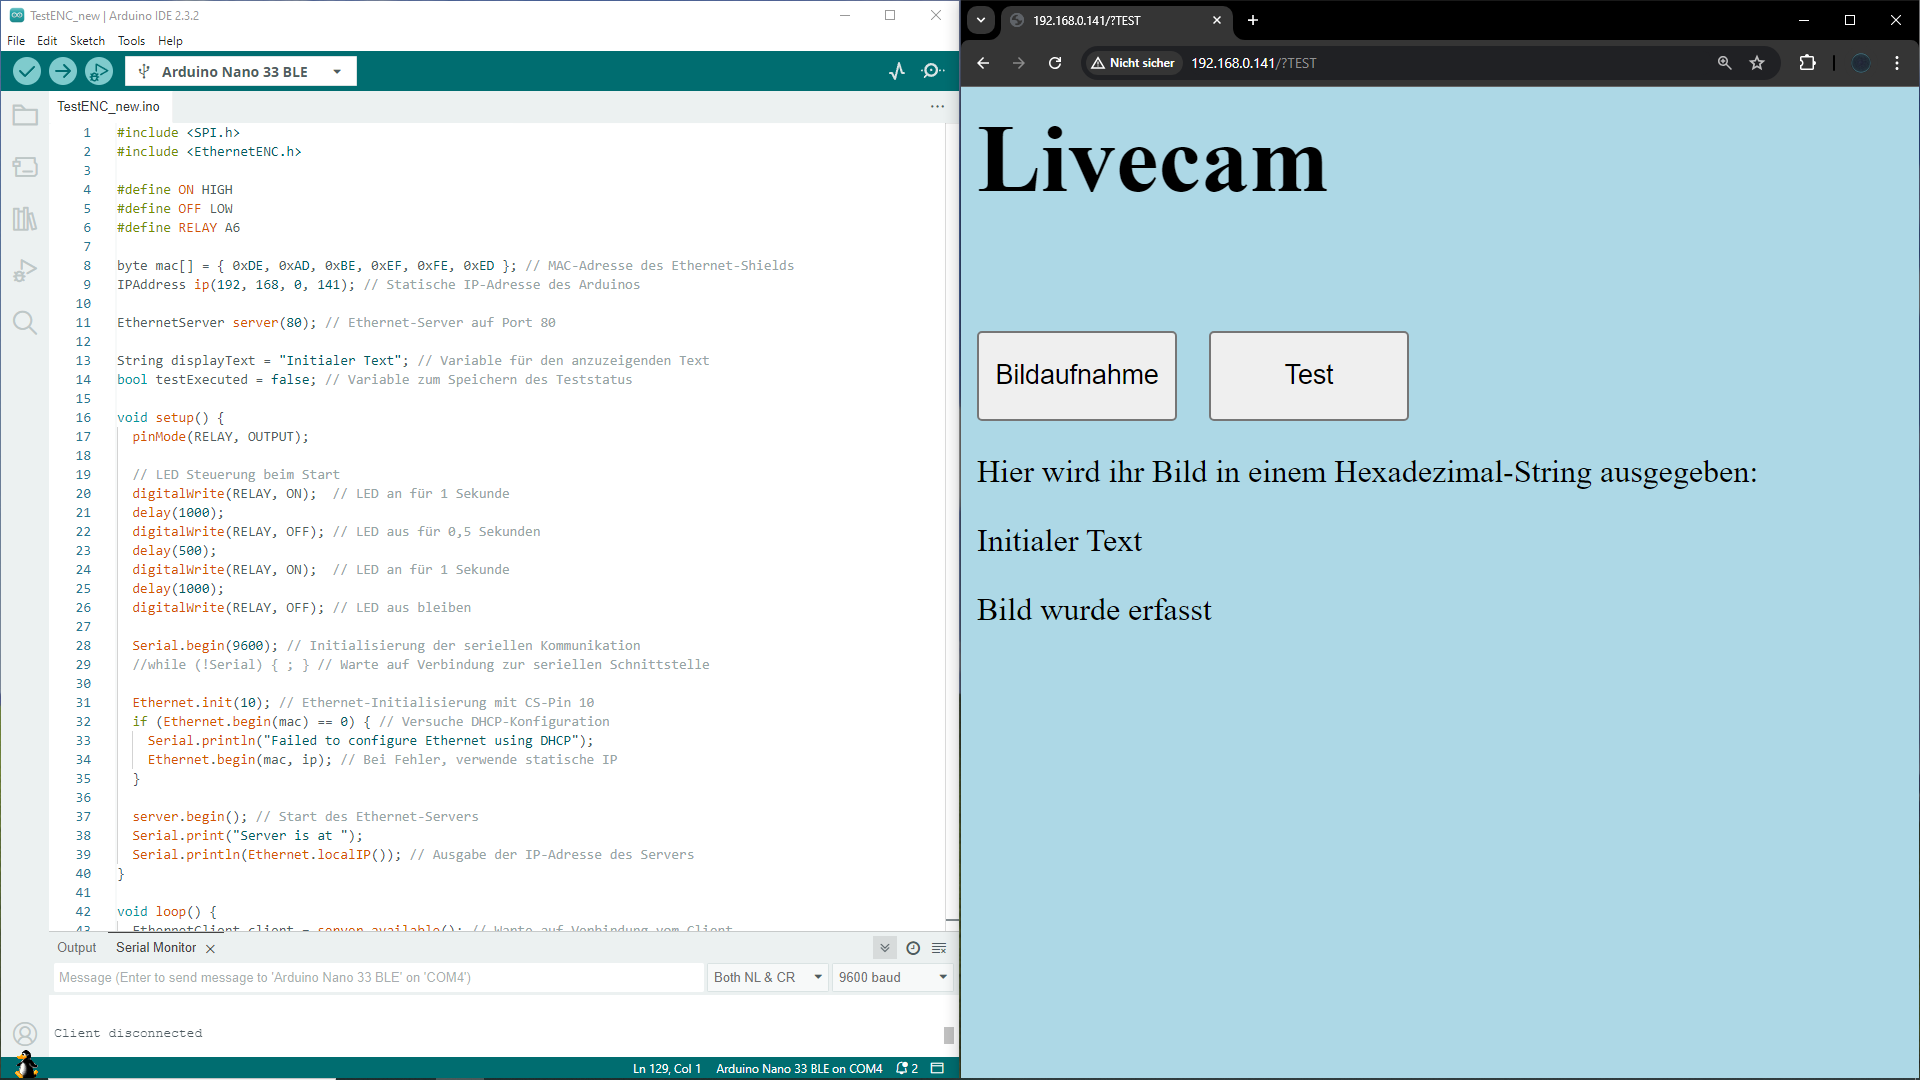
\includegraphics[width=10cm]{EthernetENC28J60/GUI}
    \caption{GUI}
    \label{fig:GUI}
\end{figure}

\begin{code}
    \lstinputlisting[language=c++]{../../Code/Arduino/EthernetENC28J60/TestENC.ino}
    \caption[Sketch \FILE{TestENC.ino}]{Der Sketch \FILE{TestENC.ino} in Arduino für das Microcontroller Board}
    \label{Code:Python:File:TestENC}   
\end{code}

\section{Datenübertragung} 

Um die Datenübertragung zu realisieren, muss die Datenmenge
verkleinert oder komprimiert werden \ref{Code:Python:File:CaptureSingleHexImage} . Zunächst wurde die Auflösung
auf 176x144 Pixel reduziert. Bei einer Farbtiefe von 16 Bit pro Pixel
entspricht das 405.504 Bits. Danach wurde von der seriellen Übertragung einzelner Bits auf die Übertragung eines
Hexadezimal-Strings umgestellt. Hexadezimalzeichenfolgen sind für Menschen besser lesbar und einfacher zu debuggen als Binärdaten. Jedes
Hexadezimalzeichen repräsentiert dabei 4 Bit, was zu einer kompakteren
und effizienteren Darstellung von Binärdaten führt.

\begin{code}
    \lstinputlisting[language=c++]{../../Code/Arduino/EthernetENC28J60/CaptureSingleHexImage.ino}
    \caption[Sketch \FILE{CaptureSingleHexImage.ino}]{Der Sketch \FILE{CaptureSingleHexImage.ino} in Arduino für das Microcontroller Board}
    \label{Code:Python:File:CaptureSingleHexImage}   
\end{code}